\documentclass[11pt]{article}
\usepackage[utf8]{inputenc}
\usepackage{amsmath,amsthm,amsfonts,amssymb,amscd}
\usepackage{multirow,booktabs}
\usepackage[table]{xcolor}
\usepackage{fullpage}
\usepackage{lastpage}
\usepackage{enumitem}
\usepackage{fancyhdr}
\usepackage{mathrsfs}
\usepackage{wrapfig}
\usepackage{setspace}
\usepackage{calc}
\usepackage{multicol}
\usepackage{cancel}
\usepackage[retainorgcmds]{IEEEtrantools}
\usepackage[margin=3cm]{geometry}
\usepackage{amsmath}
\newlength{\tabcont}
\setlength{\parindent}{0.0in}
\setlength{\parskip}{0.05in}
\usepackage{empheq}
\usepackage{framed}
\usepackage[most]{tcolorbox}
\usepackage{xcolor}
\colorlet{shadecolor}{orange!15}
\parindent 0in
\parskip 12pt
\geometry{margin=1in, headsep=0.25in}
\theoremstyle{definition}
\newtheorem{defn}{Definition}
\newtheorem{reg}{Rule}
\newtheorem{exer}{Exercise}
\newtheorem{note}{Note}
\usepackage{listings}
\usepackage{xcolor}
\usepackage{graphicx}
\setlist[itemize]{noitemsep, topsep=0pt}
\setlength{\OuterFrameSep}{0pt}
\graphicspath{ {./images/} }
\newcommand*{\Co}[2]{{}^{#1}C_{#2}}%
\lstset { %
    language=C++,
    backgroundcolor=\color{black!5}, % set backgroundcolor
    basicstyle=\footnotesize,% basic font setting
}
\NewDocumentCommand{\codeword}{v}{%
\texttt{\textbf{#1}}%
}
\begin{document}
\title{Week 1 Notes}
\thispagestyle{empty}

\begin{center}
{\vspace{5mm} \LARGE ECE 250 - Fall 2018 \\ \vspace{5mm}Aditya Arora}\\
{\vspace{5mm} \LARGE \bf Week 1 Notes}

\end{center}
\section{Introduction}

\textbf{Key details given on Course Outline, Project submissions and Policy 71}

\section{Mathematical background}
\subsection{Floor and Ceiling Functions}
Floor: The \textit{floor} function maps any real number \textit{x} onto the greatest integer less than or equal to \textit{x} 
\newline
- Consider it to be rounding towards \textit{negative infinity}
Example: floor(0.5) == 0, floor(3.2) == 3

Ceiling: The \textit{ceilling} function maps any real number \textit{x} onto the least integer integer greater than or equal to \textit{x} 
\newline
- Consider it to be rounding towards \textit{positive infinity}
Example: ceil(0.5) == 1, ceil(3.2) == 4
\newline
\begin{lstlisting}
// Both of these functions are implemented in the cmath library
# include <cmath>

double floor(double);
double ceil(double);

/*
They're double because double has a greater range (just under 2^1024) 
over long which can represent upto (2^63-1)
*/
\end{lstlisting}

\subsection{L’Hôpital’s rule}
If you are trying to determine: $\mathop {\lim }\limits_{x \to c} \frac{{f\left(x \right)}}{{g\left(x \right)}}$
but both $\mathop {\lim }\limits_{x \to c}{f\left(x \right)} = \infty$ and $\mathop {\lim }\limits_{x \to c}{g\left(x \right)} = \infty$
$$\mathop {\lim }\limits_{x \to c} \frac{{f\left(x \right)}}{{g\left(x \right)}} = \mathop {\lim }\limits_{x \to c} \frac{{f'\left(x \right)}}{{g'\left(x \right)}}$$
This rule can be repeated as necessary

\newpage

\subsection{Logarithms and Exponentials}
\begin{itemize}[label={--}]
\item If  $n = e^m$, we define
$m = ln(n)$. It is always true that $e^{ln(n)} = n$; however, $ln(e^n)$ = n requires that n is real 
\item Exponentials grow faster than any non-constant polynomial
$$\mathop {\lim }\limits_{n \to \infty}\frac{e^n}{n^d} = \infty$$ for any $d > 0$
\item Logarithms grow slower than any polynomial
$$\mathop {\lim }\limits_{n \to \infty}\frac{ln(n)}{n^d} = 0$$ for any $d > 0$
\item All logarithms are linear multiples of each other
$$log_{b}(n) = \frac{ln(n)}{ln(b)}$$
\item \begin{lstlisting}
// the base-2 logarithm log2(n) is written as lg(n)

double log(double); //ln(n)
double log10(double); //log10(n)
\end{lstlisting}
\item $m^{log_{b}(n)} = n^{log_{b}(m)}$
\end{itemize}
\newpage
\subsection{Series}
\subsubsection{Arithmetic Series}
Each term in an arithmetic series is increased by a constant value (usually 1):
$$0 + 1 + \ldots + n = \sum_{k=0}^{n} k = \frac{n(n+1)}{2}$$
$$0^2 + 1^2 + \ldots + n^2 = \sum_{k=0}^{n} k^2 = \frac{n(n+1)(2n+1)}{6}$$
$$0^3 + 1^3 + \ldots + n^3 = \sum_{k=0}^{n} k^3 = (\frac{n(n+1)}{4})^2$$
To generalise: $$\sum_{k=0}^{n} k^d \approx \int_{0}^{n} x^d dx = \frac{n^{d+1}}{d+1}$$

Absolute Error:
$$
\frac{n^d}{2} \leq \sum_{k=0}^{n} k^d - \frac{n^{d+1}}{d+1} < n^d
$$
The relative error of approximation of the equation goes to zero as $n$ tends to $\infty$

\subsubsection{Geometric Series}
The next series we will look at is the geometric series with common ratio r:
$$\sum_{k=0}^{n} r^k = \frac{1-r^{n+1}}{1-r}$$
and if $|r| < 1$ then it is also true that
$$\sum_{k=0}^{\infty} r^k = \frac{1}{1-r}$$

\newpage
\subsection{Recurrence Relations}
\begin{itemize}[label={--}]
\item A recurrence relationship is a means of defining a sequence based on previous values in the sequence.
\item Such definitions of sequences are said to be \textit{recursive}
\begin{shaded}
Define an initial value: e.g., $x_1 = 1$
\newline
Defining $x_n$ in terms of previous values:
For example,
	  		$$x_n = x_{n – 1} + 2$$
			$$x_n = 2x_{n – 1} + n$$
			$$x_n = x_{n – 1} + x_{n – 2}$$
\end{shaded}
\end{itemize}
\subsection{Weighted Average}
Given n objects $x_1, x_2, x_3, \ldots, x_n$, the average is
$$\frac{x_1+x_2+x_3\ldots+x_n}{n}$$
	Given a sequence of coefficients $c_1 , c_2 , c_3 ,\ldots, c_n$ where
$$c_1 + c_2 + \ldots + c_n = 1$$
then we refer to:
$$\frac{c_1x_1+c_2x_2+c_3x_3\ldots+c_nx_n}{n}$$	as a weighted average \newline
For an average, $c_1 = c_2 = \ldots = c_n = 1$
\newline
Examples:
\newline
\begin{minipage}{0.4\textwidth}
\begin{itemize}[label={--}]
\item Simpson’s method approximates an integral by sampling the function at three points:  f(a), f(b), f(c)
\item The average value of the function is approximated by
\end{itemize}
\end{minipage}%
%
\begin{minipage}{0.4\textwidth}
\begin{center}
    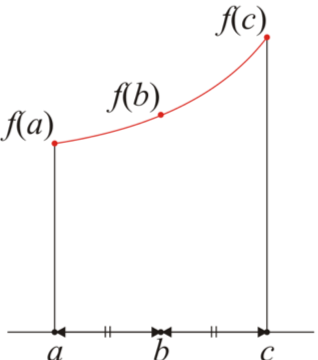
\includegraphics[width=0.6\textwidth]{simmons}
    \label{img:g}
\end{center}
\end{minipage}

\newpage
\subsection{Combinations}
Given n distinct items, in how many ways can you choose k of these?
The number of ways such items can be chosen is written:
$$\Co{n}{k} = \frac{n!}{(k!)(n-k)!}$$

This is also a recursive definition:
$\Co{n}{k} = \Co{n-1}{k} + \Co{n-1}{k-1}$

\begin{itemize}[label={--}]
\item These are also the co-efficients of Pascal's Triangle
\item They are also the coefficients that we use to expand $(x+y)^n$
\end{itemize}

\newpage
\section{A Brief Introduction to C++}

\subsection{Operators}
\begin{lstlisting}
Assignment	        =

Arithmetic		+     -     *     /     %
			+=    -=    *=    /=    %=
			
Autoincrement	        ++
Autodecrement	        --

Logical		        &&      ||    !

Relational	        ==    !=    <     <=    >=    >

Comments	        /*  Block Comments 
                            over multiple lines */
		        // to end of line
			
Bitwise		        &     |     ^     ~
			&=    |=    ^=
				
Bit shifting	        <<    >>
			<<=   >>=
\end{lstlisting}
\subsection{Control Statements}
\begin{lstlisting}
/* Conditionals */

if(statement){
    something;
}
else if(statement2){
    something_else;
}
else{
    finally_something;
}

/* Loops */

// for loop
for(int i = 0; i < n; i++){
    statement[i] = i;
}

// while loop
while(statement){
    something;
}

// do while
do{
    something;
}while(statement)

\end{lstlisting}
\newpage
\subsection{Printing}
Printing to console in C++ is done by overloading the \codeword{<<} operator.

If the left-hand argument of \codeword{<<} is an object of type \codeword{<<} ostream (output stream) and the right-hand argument is a double, int, string, or even a custom defined class (provided you have defined a method inside the class to handle this,) an appropriate function which prints the object is called
\begin{lstlisting}
cout << "The square of 3 is " << sqr(3) << endl;
// prints string + int + end of line identifier
// the line above is equivalent to:
((cout << "The square of 3 is ") << sqr(3)) << endl;
// or
operator<<(operator<<(operator<<(cout, "The square of 3 is "), sqr(3)), endl);
\end{lstlisting}
\subsection{Arrays}
\begin{lstlisting}
const int ARRAY_CAPACITY = 10; // const prevents reassignment
int array[ARRAY_CAPACITY]; 
 /* for any number to be used as a size of an array it has to be a const */
array[0] = 1; // setting first element to be 1

for (int i = 0; i < ARRAY_CAPACITY; ++i) {
    // arrays go from 0 to ARRAY_CAPACITY-1
    array[i] = 2*array[i-1] + 1;
}
\end{lstlisting}
\begin{itemize}[label={--},nolistsep]
    \item The \textbf{capacity} of an array is the entries it can hold
    \item The \textbf{size} of an array is the number of useful entries 
\end{itemize}
\subsection{Functions}
\begin{lstlisting}
// A function with a global name
int sqr(int n){
    return n*n;
}

int main(){
    cout << "The square of 3 is " << sqr(3) << endl;
    return 0;
}
\end{lstlisting}
\newpage
\subsection{Pre-processing statements}
Any command starting with a \# in the first column is not a C/C++ statement, but rather a preprocessor statement

The preprocessor performs very basic text-based (or lexical) substitutions and the output of which is sent to the compiler

The preprocessor just copy pastes the code from the source file to the file where it is called
\begin{lstlisting}
// Guard statements ensure that we don't import the same file twice

#ifndef SINGLE_LIST_H
#define SINGLE_LIST_H

template <typename Type>

class Single_list {
	///...
};
#endif
\end{lstlisting}
\subsection{Compilation}
In C/C++, the file is the base unit of compilation. Any .cpp file may be compiled into object code
Only files containing an int main() function can be compiled into an executable
\begin{lstlisting}
int main () {
    // does some stuff
    return 0;
}
\end{lstlisting}
The operating system is expecting a return value from \codeword{int main()} which is usually 0. Functions called in \codeword{int main()} can originate from other files which can be \codeword{#include}(d)
\newpage
\subsection{Namespaces}
Namespaces can help us differentiate between scopes of variables, functions and classes. 

Variables defined:
\vspace{-4mm}
\begin{itemize}[label={--},topsep=0pt]
    \item In functions are \textit{local} variables
    \item In classes are \textit{member} variables
    \item Elsewhere are \textit{global} variables
\end{itemize}
Functions defined:
\vspace{-4mm}
\begin{itemize}[label={--},topsep=0pt]
    \item In classes are \textit{member} functions
    \item Elsewhere are \textit{global} functions
\end{itemize}
A namespace adds an extra disambiguation between similar names
\begin{lstlisting}
namespace a{
    int n = 3;
    void test(){
        int a = 3, b = 5;
        cout << a + b;
    }
}
// To access variables and functions inside a namespace there are 2 methods:

// first method using scope operator (::)
cout << a::n;

// second method using keyword using
using namespace a; /* this maintains the namespace in the 
                      following lines until you change it */
test(); // no need for scope operator

/* 
The default namespace is std, 
all variables and functions in the 
standard library are in the std namespace 
*/
using namespace std; 
\end{lstlisting}
\newpage
\subsection{Classes}

\begin{minipage}{0.3\textwidth}
A way to summarize the properties of a class is through UML Class Diagrams.
\\
UML, the Unified Modeling Language is a collection of best practices used in designing/modeling (among other things) software systems
\end{minipage}%
%
\begin{minipage}{0.7\textwidth}
\begin{center}
    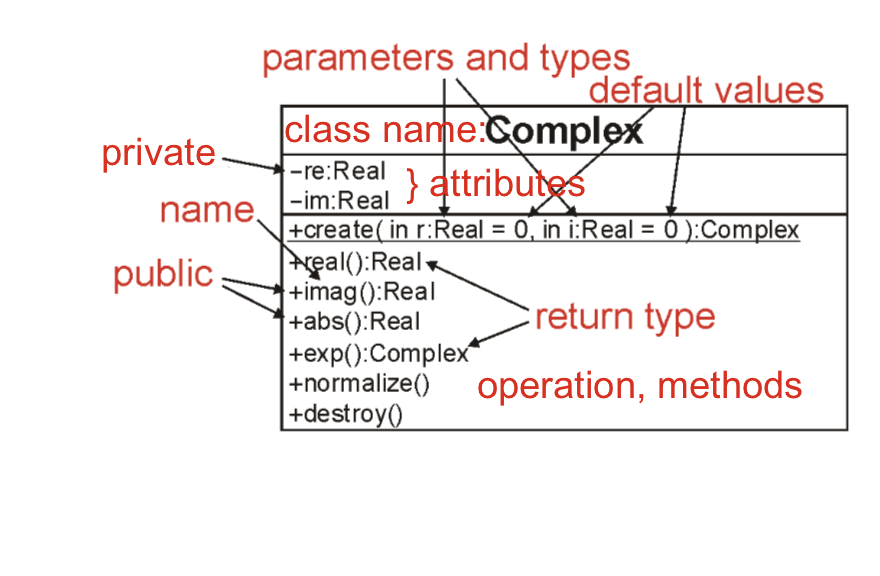
\includegraphics[width=0.7\textwidth]{uml2}
    \label{img:g}
\end{center}
\end{minipage}

\begin{lstlisting}
// Class declaration, does not include the implementation
#ifndef _COMPLEX_H
#define _COMPLEX_H
#include <cmath>

class Complex {

    private:
        double re, im;

    public:
        Complex(double = 0.0, double = 0.0);

        // Accessors
        double real() const;
        double imag() const;
        double abs() const;
        Complex exp() const;

        // Mutators
        void normalize();
};
\end{lstlisting}
\newpage
\begin{lstlisting}
// Class Implementation:
Complex::Complex(double r, double i):re(r),im(i){} 
// For built in data-types the above constructor is equal to
Complex::Complex(double r, double i):re(0), im(0){
    re = r;
    im = i;
}

// return the real component
double Complex::real() const {
    return re;
}

// return the imaginary component
double Complex::imag() const {
    return im;
}

// return the absolute value
double Complex::abs() const {
    return std::sqrt(re*re + im*im);
}

// Return the exponential of the complex value
Complex Complex::exp() const {
    double exp_re = std::exp(re);
    return Complex(exp_re*std::cos(im), exp_re*std::sin(im));
}

// Normalize the complex number (giving it unit absolute value, |z| = 1)
void Complex::normalize() {
    if (re == 0 && im == 0) {
        return;
    }

    double absval = abs(); // calls the abs function declared above
    re /= absval;
    im /= absval;
}

#endif
\end{lstlisting}
\newpage
\subsubsection{Visibility}
\begin{lstlisting}
class ClassY;                   // declare that ClassY is a class
class ClassX {
    private:
        int privy;              // the variable privy is private

    friend class ClassY;        // ClassY is a "friend" of ClassX
};

class ClassY {                  // define ClassY
    private:
        ClassX value;           // Y stores one instance of X

    public:
        void set_x() {
            value.privy = 42;   // a member function of ClassY can
        }                       // access and modify the private
};   
\end{lstlisting}
\subsubsection{Accessors and Mutators}
\textbf{Accessors}:	we are accessing and using the class members\\
\textbf{Mutators}: we are changing—mutating—the class members

Good programming practice is to enforce that a routine specified to be an accessor cannot be accidentally changed to a mutator
This is done with the const keyword after the parameter list \lstinline{double abs() const;}
\subsubsection{Templates}
To build a general class which extends to all data types we use a different mechanism, using a tool called templates\\
- A function has parameters which are of a specific type\\
- A template is like a function, however, the parameters themselves are types
\begin{lstlisting}
#include<iostream>
using namespace std;

template <typename Type>
Type sqr(Type x) {
    return x*x;
}
	
int main() {
    cout << "3 squared is " << sqr<int>(3) << endl;
cout << "Pi squared is " << sqr<double>(3.141592653589793) << endl;
return 0;
}
\end{lstlisting}
\newpage
\begin{lstlisting}
#ifndef _COMPLEX_H
#define _COMPLEX_H
#include <cmath>
template <typename Type>

class Complex {

    private:
        Type re, im;

    public:

        Complex(Type const & = Type(), Type const & = Type());
        
        // Accessors
        Type real() const;
        Type imag() const;
        Type abs() const;
        Complex exp() const;

        // Mutators
        void normalize();
};

// Constructor
template <typename Type> 
/*The modifier template <typename Type> applies only 
to the following statement, so each time we define a 
function, we must restate that Type is a templated symbol:*/

Complex<Type>::Complex(Type const &r, Type const &i):re(r), im(i) {
    // empty constructor
}

// return the real component
template <typename Type>
Type Complex<Type>::real() const {
    return re;
}

// return the imaginary component
template <typename Type>
Type Complex<Type>::imag() const {
    return im;
}

// return the absolute value
template <typename Type>
Type Complex<Type>::abs() const {
    return std::sqrt(re*re + im*im);
}

// return the exponential of the complex value
template <typename Type>
Complex<Type> Complex<Type>::exp() const {
    Type exp_re = std::exp(re);
    return Complex<Type>(exp_re*std::cos(im), exp_re*std::sin(im));
}

// normalize the complex number (giving it unit norm, |z| = 1)
template <typename Type>
void Complex<Type>:noramlize() {
    if (re == 0 && im == 0) {
        return;
    }

    Type absval = abs();
    re /= absval;
    im /= absval;
}

#endif
\end{lstlisting}
\begin{lstlisting}
// using the template files
#include <iostream>
#include "Complex.h"

using namespace std;

int main() {
    Complex<double> z(3.7, 4.2);
    Complex<float>  w(3.7, 4.2);
    cout.precision(20); // Print up to 20 digits
    
    cout << "|z| = " << z.abs() << endl;
    cout << "|w| = " << w.abs() << endl;

    z.normalize();
    w.normalize();

    cout << "After normalization, |z| = " << z.abs() << endl;
    cout << "After normalization, |w| = " << w.abs() << endl;

    return 0;
}
\end{lstlisting}
\newpage
\subsection{Pointer}
- Every variable (barring optimization) is stored somewhere in memory\\
- That address is an integer, so we can store the address the in a variable
\newline
We could simply have an ‘address’ type: \codeword{address ptr;} however, the compiler does not know what it is an address of (is it the address of an int, a double, etc.)
Instead, we have to indicate what it is pointing to:
\begin{lstlisting}
int *ptr;   // a pointer to an integer, the address of the integer variable 'ptr'
int m = 5;    // m is an int storing 5
ptr = &m;     // assign to ptr the address of m
cout << ptr << endl; //	prints 0xffffd352, a 32-bit number
// note: the computer uses 32-bit addresses
// access/modify what is stored at that memory location by using the * operator
cout << *ptr << endl; // prints 5
*ptr = 3;    // store 3 at that memory location 
cout << m << endl;  // prints 3
\end{lstlisting}
\begin{lstlisting}
// pointers to objects must, similarly be dereferenced:
Complex z( 3, 4 );
Complex *pz;
pz = &z;
cout << z.abs() << endl;
cout << (*pz).abs() << endl;
// shorthand pz->abs() == (*pz).abs()
cout << pz->abs() << endl;
\end{lstlisting}
\subsection{Memory Allocation}
Memory allocation in C++ and C\# is done through the \codeword{new} operator\\
This is an explicit request to the operating system for memory
This is a very expensive operation\\
The OS must:\\
- Find the appropriate amount of memory,\\
- Indicate that it has been allocated, and\\
- Return the address of the first memory location
C++ requires the user to explicitly de-allocate memory, For each new, there must be a corresponding delete\\
\begin{shaded}
Note:\\
- managed C++ has garbage collection\\
- other tools are also available for C++ to perform automatic garbage collection
\end{shaded}
Inside a function, memory allocation of declared variables is dealt with by the compiler automatically
Memory for a single instance of a class (one object) is allocated using the new operator, e.g.,
\begin{lstlisting}
Complex<double> *pz = new Complex<double>( 3, 4 );
cout << "The address pz is " << pz << endl; // The address pz is 0x00ef3b40
// new operator returns the address of the first byte of the memory allocated 
delete pz; // de-allocates the memory
\end{lstlisting}

\end{document}
